\chapter{Robustness of core-periphery algorithm} % Main chapter title
\label{App:robust}
\textbf{Precision and recall}

Consider the network $G(V, L)$, with a set of nodes $V$ and a set of links between them $L$. The stochastic community detection algorithms may converge to different configurations. To quantify the similarity between the obtained structures and the algorithm's robustness, we run 50 iterations and calculate several similarity measures between pairwise partitions $C$ and $C^{'}$.

The core-periphery structure has two groups, so confusion matrix \cite{labatut2012accuracy} can be defined as:

\begin{center}
	
	\begin{tabular}{l|l|c|c|c} 
		
		\multicolumn{2}{c}{}&\multicolumn{2}{c}{partition C}&\\ 
		
		\cline{3-4} 
		\multicolumn{2}{c|}{}&core&periphery&\multicolumn{1}{c}{}\\
		\cline{2-4} 
		partition & core & $n_{TP}$ & $n_{FN}$ & \\ 
		\cline{2-4} $C^{'}$ & periphery & $n_{FP}$ & $n_{TN}$ & \\ 
		\cline{2-4}
	\end{tabular}
\end{center}

The diagonal elements correspond to the number of nodes found in the same class in both node configurations. The number of nodes in the core found in $C$ and $C^{'}$ is denoted as true positive $n_{TP}$, while the number of nodes in the periphery in $C$ and $C^{'}$ is denoted as true negative $n_{TN}$. The off-diagonal elements of the confusion matrix indicate the number of nodes differently classified. We can define the number of nodes found in the first configuration C in the core but in $C^{'}$ in the periphery as a false positive, $n_{FP}$, similarly the number of nodes found in the periphery in the partition $C$, and in the core in partition $C^{'}$ as a false positive, $n_{FP}$. 

From the confusion matrix, we can write the precision $P =n_{TP}/(n_{TP}+n_{FP})$ and recall $R=n_{TN}/(n_{TN}+n_{FN})$. These measures range from 0 to 1. The precision (recall) corresponds to the proportion of instances predicted to belong (not belong) to the considered class and which indeed do (do not) \cite{labatut2012accuracy}.

The \textbf{F1 measure} is the harmonic mean of precision and recall \cite{labatut2012accuracy}:
\begin{equation}
F_1 = 2\frac{P \cdot R}{P+R} = \frac{2n_{TP}}{2n_{TP}+n_{FN} + n_{FP}}.
\end{equation}
It can be interpreted as a measure of overlap between true and estimated classes; it is 0 for no overlap to 1 if the overlap is complete.

The \textbf{Jaccard's} coefficient is the ratio of two classes' intersection to their union \cite{labatut2012accuracy}. It can also be expressed in terms of a confusion matrix: 
\begin{equation}
J =  \frac{C_{core} \cap C^{'}_{core}}{C_{core} \cup C^{'}_{core}} =   \frac{n_{TP}}{n_{TP}+n_{FP} + n_{FN}}.
\end{equation}

\textbf{Normalized mutual information (NMI)} is similarity measure between to partitions $C$ and $C^{'}$  based on information theory \cite{danon2005comparing}:

\begin{equation}
NMI(C, C^{'}) = \frac{MI(C, C^{'})}{(H(C)+H(C^{'})/2}.
\end{equation}

where $MI$ is mutual information between sets $C$ and $C^{'}$, while $H(C)$ is entropy of given partition. The entropy is defined as $H(C) = - \sum_{i=1}^{|C|}P(i)log(P(i))$, where $P(i) = |U_i|/N$ is the probability that an object is randomly classified as $i$ (in this special case $i=0$, the node belongs to the core, or $i=1$, the node belongs to the periphery). The mutual information between sets $C$ and $C^{'}$ measures the probability that the randomly chosen node is a member of the same group in both partitions:
\begin{equation}
MI(C, C) = \sum_i\sum_j P(i, j) log(\frac{P(i,j)}{P(i)P^{'}(j)})    .
\end{equation}
where $P(i, j)= |U_i \cap U_j|/N$.

$NMI$ ranges from 0 when the partitions are independent to 1 if they are identical.   

\textbf{Adjusted rand index.} For the set of nodes $V$, with $n$ nodes, consider all possible combination of pairs $(v_i, v_j)$. We can select the number of the pairs where nodes belong to the same group in both partitions, $C$ and  $C^{'}$, denoted as $a$. Similarly, as $b$, we can define the number of pairs whose nodes belong to different groups in partitions. Then, unadjusted rand index \cite{santos2009use} is given as $RI = \frac{a+b}{\binom{n}{2}}$, where $\binom{n}{2}$ is number of all possible pairs. The RI between two randomly assigned partitions is not close to zero; for that reason, it is common to use the adjusted rand index \cite{hubert1985comparing}, defined as:
\begin{equation}
ARI = \frac{RI - E[RI]}{max(RI)- E[RI]},
\end{equation}
where $E[RI]$ is expected value of RI, and $max(RI)$ is maximum value of $RI$. 

\clearpage
For example, we show an analysis of an inferred sample of core-periphery structures for 30 days of closed Astronomy, Stack Exchange networks, Figure \ref{fig:sample}. We represent the mean minimum description length (MDL) and the mean number of nodes in the core with standard deviation. MDL does not change much between inferred core-periphery structures; the difference between obtained configurations is still notable in the number of nodes in the core. To investigate the similarity between obtained core-periphery configurations in the sample more deeply, we calculate several measures between pairwise partitions, such as normalized mutual information, adjusted rand index, F1 measure and Jaccard index. These measures are greater than 0.5 and, in most cases, greater than 0.9, indicating the stability of the inferred core-periphery structures.


\begin{figure}[h]
	\centering
	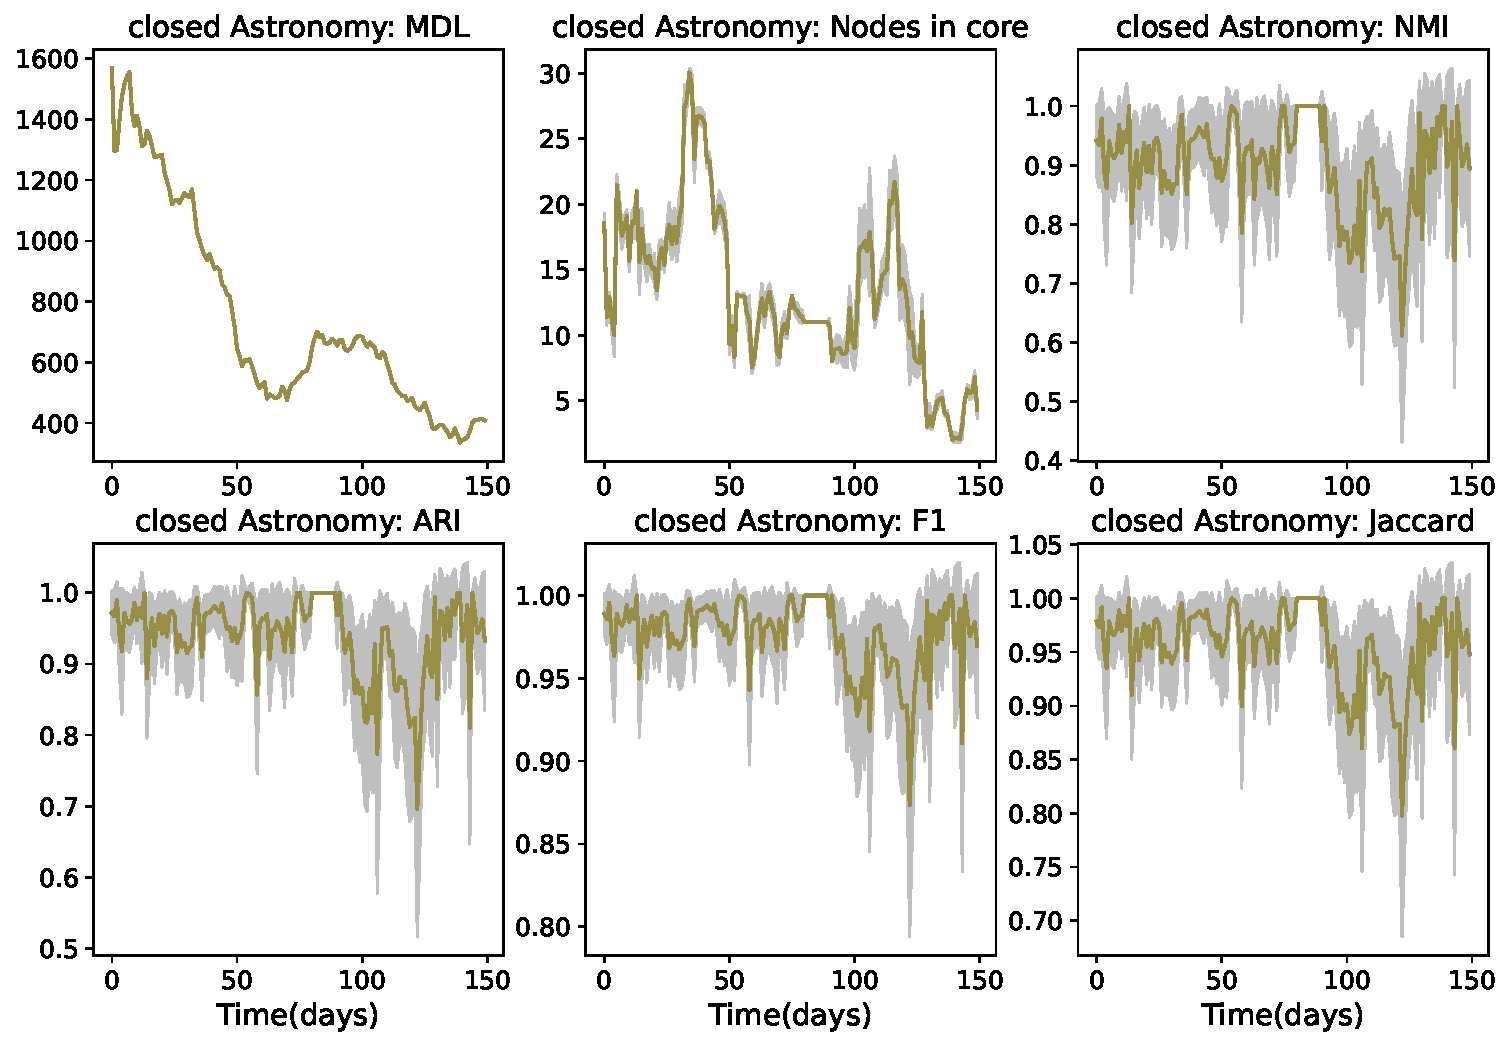
\includegraphics[width=0.8\linewidth]{appendixD/blockmodel_robust.pdf}
	\caption[Stability of the core-periphery structures.]{Minimum description length, number of nodes in the core, normalized mutual information, adjusted rand index, F1 measure and Jaccard index, among 50 samples for 30-days sub-networks. Results are given for closed astronomy. }
	\label{fig:sample}
\end{figure}